\chapter{El zoológico de las variables aleatorias, parte 1}
\labch{zoologico1}

En el mundo\sidenote{realidad, naturaleza, universo, cosmos o como quiera llamarlo según su tendencia filosófica} hay una infinidad y variedad de hechos que podrían estudiarse como variables aleatorias. En principio, deberíamos estudiar cada uno de ellos de manera individual, pero no cuesta mucho ver que eso sería demasiado difícil. Además, podemos abstraer detalles para quedarnos con los hechos que marcan más presencia.

De esta manera podemos llegar a varios \emph{modelos de probabilidad} para estudiar diversas variables aleatorias. En este capítulo estudiaremos varios modelos discretos, bajo qué condiciones se pueden aplicar y qué tipo de \va\ quieren modelar. En el siguiente capítulo continuaremos nuestro paseo pero por modelos continuos. Si bien estudiaremos varias distribuciones, hay varias más que quedarán fuera del alcance de este curso. Para los y las interesados, eventualmente habrá un apéndice con alguna descripción de estas distribuciones.

\section{Distribución de Bernoulli}
\labsec{bernoulli}

Probablemente el modelo de probabilidad más sencillo, la distribución de Bernoulli (o dicotómica) es una con la que, para ser sinceros, nos encontramos desde la primera clase.

Si tenemos un experimento aleatorio, podemos entender su resultado desde el punto de vista de \emph{éxito} o fracaso. El ejemplo clásico es la moneda. Queremos que salga cara y, si sale cara, tenemos un éxito. Si sale sello, tenemos un fracaso.

Pero fenómenos más complejos se pueden reducir a esta perspectiva de éxito-fracaso. Me encantó el ejemplo que dio un estudiante: quiero que mi equipo gane el partido. Si no gana (pierda o empate), eso es un fracaso. Imagínense estudiar eso desde el punto de vista de todos los resultados posibles (0-0, 1-0, 0-1, 1-1, 2-0,\ldots). Una locura.

Incluso, este lenguaje de éxito-fracaso puede ser todo lo contrario en la realidad. Puedo definir mi éxito como encontrar un resultado positivo en un examen, lo que seguramente para el paciente sería algo negativo, porque sugeriría\sidenote{después del capítulo de Bayes, ya no podemos decir \enquote{confirmaría}} que tiene la enfermedad.

En resumen, tenemos algún tipo de evento aleatorio. Ese evento tiene un conjunto de resultados. Definiremos algunos como éxito y el resto como fracaso. De esta manera, definiremos la variable aleatoria
\[X=\begin{cases}
    1 & \text{éxito}\\
    0 & \text{fracaso.}
\end{cases}\]

Además, la probabilidad de esta variable aleatoria será
\[\prob(X=x)=\begin{cases}
    p&x=1\\
    1-p=q&x=0.
\end{cases}\]
Es muy usual esta notación de \(q=1-p\) para la probabilidad del fracaso. En lo que queda de los apuntes intentaré usarla. 

La distribución de Bernoulli en sí misma no es muy interesante, pero la importancia que tiene es que varias distribuciones que sí son interesantes están relacionadas con ella. Pero antes de entrar a eso, cerremos nuestro estudio de esta distribución y veamos su esperanza y  varianza.

La esperanza es muy fácil de calcular
\[\esp{X} = \sum_{x=0}^{1}x\prob(X=x)=0\cdot q+ 1\cdot p = p.\] Es decir, la esperanza de \(X\) es \(p\). La varianza es
\begin{align*}
    \sigma^2 &= \esp{X^2}-\esp{X}^2\\
    &= \sum_{x=0}^{1}x^2\prob(X=x) - p^2\\
    &= 0^2\cdot q + 1^2\cdot p - p^2\\
    &= p-p^2\\
    &= p(1-p) = pq
\end{align*}

Estos resultados nos servirán más adelante.

\section{Variables aleatorias discretas y su relación con \va s Bernoulli}
\labsec{relacion-bernoulli}

Una \va\ Bernoulli representa el éxito o fracaso en \emph{una} repetición de un experimento aleatorio. Pero si repetimos el mismo experimento varias veces bajo las siguientes condiciones
\begin{enumerate}
\item cada repetición es independiente y
\item la probabilidad de éxito se mantiene constante
\end{enumerate}
tenemos tres tipos de \va s que aparecen naturalmente.

Una posibilidad es preguntarnos por la probabilidad de tener \(k\) éxitos si repetimos el experimento \(n\) veces, donde \(n\) es un número fijo y \(k\) va entre 0 y \(n\). Esta pregunta da origen a la distribución de probabilidad \emph{binomial.}

Otra posibilidad es preguntarnos cuánto nos demoraremos en tener nuestro primer éxito. Esta pregunta da origen a la distribución de probabilidad \emph{geométrica.}

Una tercera posibilidad es preguntarnos cuánto nos demoraremos en obtener un cierto número (fijo) de éxitos. Esta pregunta da origen a la distribución \emph{binomial negativa.}

Estas relaciones aparecen resumidas en la \reffig{relacion-bernoulli}.

\begin{figure*}
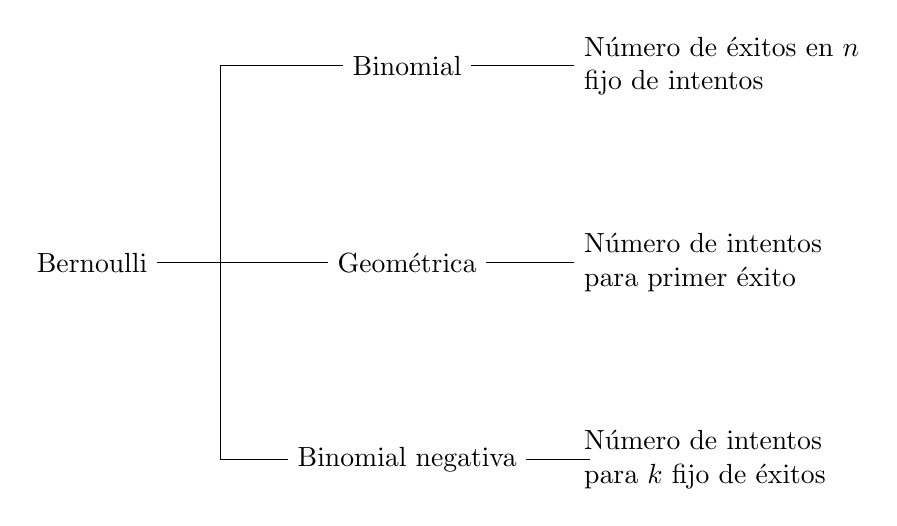
\begin{tikzpicture}[
    grow=right,
    level distance=4cm,
    level 1/.style={sibling distance=2.5cm},
    edge from parent path={(\tikzparentnode.east) -- ++(0.8cm,0) |- (\tikzchildnode.west)},
    every node/.style={align=left}
]
\node {Bernoulli}
    child { node {Binomial negativa} 
        child { node[text width=3.5cm] {Número de intentos para \(k\) fijo de éxitos} }
    }
    child { node {Geométrica} 
        child { node[text width=3.5cm] {Número de intentos para primer éxito} }
    }
    child { node {Binomial} 
        child { node[text width=3.5cm] {Número de éxitos en \(n\) fijo de intentos} }
    };
\end{tikzpicture}
\caption{Relación entre las variables aleatorias Bernoulli y algunas variables aleatorias discretas.}
\labfig{relacion-bernoulli}
\end{figure*}

Existe otra relación. ¿Qué pasa si relajamos la necesidad de independencia? Podemos imaginar que tenemos el experimento aleatorio de sacar pelotas de una caja. Con reposición significa que lo hacemos con independencia, porque las probabilidades vuelven a ser las mismas. Pero si lo hacemos sin reposición, las probabilidades van cambiando. En este caso, la distribución de probabilidad que surge al preguntarnos cuál es la probabilidad de tener \(k\) éxitos en \(n\) intentos es la distribución \emph{hipergeométrica.}

Una última relación que podemos establecer es cuando tenemos una cantidad promedio fija de eventos independientes que ocurren en una unidad de tiempo (o espacio, área, volumen, etc.). Por ejemplo, si siempre me llegan en promedio 10 correos de spam por hora, podría calcular la probabilidad de que me lleguen 40 en un día. O, si revuelvo de manera suficientemente buena mi masa, la probabilidad de que la galleta que me voy a comer tenga 5 chips de chocolate si en promedio tienen 3. Eventos de este tipo se modelan con una distribución de Poisson. 

Hay una relación entre la distribución binomial y la de Poisson. Si hacemos muchos intentos (\(n\to\infty\)) y la probabilidad de éxito de cada uno es pequeña (\(p\to0\)) pero de manera que \(np=\lambda\) sea constante, entonces la distribución de Poisson aparece como un límite de la distribución binomial.

% \begin{tikzpicture}[
%     scale=0.9,
%     transform shape,
%     grow=right,
%     level distance=4cm,
%     level 1/.style={sibling distance=2.8cm},
%     edge from parent path={(\tikzparentnode.east) -- ++(0.7cm,0) |- (\tikzchildnode.west)},
%     every node/.style={align=left, font=\small}
% ]
% \node {Poisson}
%     child { node[text width=3.2cm] {Cadena de\\aproximaciones}
%         child { node[text width=4.2cm] {Hipergeométrica $\to$ Binomial $\to$ Poisson} }
%     }
%     child { node[text width=3.2cm] {Aproximación a\\Binomial negativa}
%         child { node[text width=4.2cm] {Eventos raros en muchos intentos} }
%     }
%     child { node {Proceso de Poisson}
%         child { node[text width=4.2cm] {Eventos en intervalo $\to$ Poisson,\\
%                                        Tiempo entre eventos $\to$ Exponencial,\\
%                                        Tiempo hasta $k$-ésimo evento $\to$ Gamma/Erlang} }
%     }
%     child { node {Suma de Poisson}
%         child { node[text width=4.2cm] {$X_1+X_2 \sim \text{Poisson}(\lambda_1+\lambda_2)$} }
%     }
%     child { node[text width=3.2cm] {Límite de la\\Binomial}
%         child { node[text width=4.2cm] {Cuando $n\to\infty$, $p\to 0$, $np=\lambda$} }
%     };
% \end{tikzpicture}

Con eso, entremos más en detalle en cada una de ellas.

\section{Distribución binomial}
\labsec{binomial}

Como se dijo en la sección anterior, la distribución binomial modela la probabilidad de obtener \(k\) éxitos en \(n\) repeticiones independientes de un experimento con probabilidad de éxito \(p\). En este caso, \(n\) es un número fijo que se asume sabido de antemano. \(p\) también es un número sabido de antemano. Decimos entonces que \(n\) y \(p\) son \emph{parámetros}\sidenote{la mejor definición de parámetro se la escuché a un físico: una constante que varía} de nuestra distribución. 

Pensemos qué significa esto. Si tenemos \(n\) intentos y queremos obtener \(k\) éxitos, tendremos \(n-k\) fracasos. La probabilidad que esto ocurra, sabiendo que cada repetición es independiente es, por lo tanto, \[p^kq^{n-k}.\] Sin embargo, ¿de cuántas maneras podemos tener esa cantidad de éxitos y fracasos? Recordando lo que aprendimos en la sección \nrefsec{conteo}, esto es equivalente a obtener \(k\) elementos de un conjunto con \(n\) elementos sin que nos importe el orden \[\binom{n}{k}.\]

Con esto, entonces, si \(X\) es una variable aleatoria con distribución de probabilidad binomial, la probabilidad de obtener \(k\) éxitos en \(n\) lanzamientos viene dada por \[\prob(X=k) = \binom{n}{k}p^kq^{n-k}.\] Además, simbolizaremos la idea de que la distribución de probabilidad de \(X\) es binomial con parámetros \(n, k\) como\marginnote{el símbolo \(\sim\) significa que la variable aleatoria se distribuye como dice la función de la derecha} \[X\sim\Bin(n, p).\]

Exploremos algunos gráficos para entender cómo se ve esta distribución. En la  \reffig{binomial-varios-p} vemos la distribución binomial para \(n=20\) y varios valores de \(p\). Vemos que, para \(p\) pequeño, la distribución está \enquote{cargada} a la izquierda. Para \(p\) grande, está \enquote{cargada} a la derecha. Y para \(p=0.5\), es simétrica.

Por otra parte, en la \reffig{binomial-varios-n} vemos la distribución binomial para \(p=0.3\) y varios valores de \(n\). La distribución, al aumentar \(n\) se va \enquote{expandiendo}.

\begin{figure*}
\centering
% Binomial pmf plots for n=20 and p in {0.2, 0.5, 0.8}
\begin{tikzpicture}
\begin{groupplot}[
  group style={group size=3 by 1, horizontal sep=1cm},
  width=0.6\textwidth, height=0.24\textheight,
  xmin=-0.5, xmax=20.5,
  ymin=0, ymax=0.22,
  yticklabel style={/pgf/number format/fixed},
  xtick={0,5,10,15,20},
  xlabel={$k$},
  ylabel={},
  enlargelimits=false,
  ymajorgrids,
  axis lines = middle,
  ybar,
axis y line=none,
ytick=\empty,
ymajorgrids=false,
ylabel={}
]
  % p = 0.2
  \nextgroupplot[title={$p=0.2$}]
  \addplot+[bar width = 2pt, samples at={0,...,20}] {binompdf(x,20,0.2)};

  % p = 0.5
  \nextgroupplot[title={$p=0.5$}]
  \addplot+[bar width = 2pt, samples at={0,...,20}] {binompdf(x,20,0.5)};

  % p = 0.8
  \nextgroupplot[title={$p=0.8$}]
  \addplot+[bar width = 2pt, samples at={0,...,20}] {binompdf(x,20,0.8)};
\end{groupplot}
\end{tikzpicture}
\caption{Distribución binomial con $n=20$ y distintos $p$.}
\labfig{binomial-varios-p}
\end{figure*}

\begin{figure*}
\centering
% Binomial pmf plots for p=0.3 and n in {5, 10, 20}
\begin{tikzpicture}
\begin{groupplot}[
  group style={group size=3 by 1, horizontal sep=1cm},
  width=0.6\textwidth, height=0.24\textheight,
  xmin=-0.5, xmax=20.5,
  ymin=0, ymax=0.22,
  yticklabel style={/pgf/number format/fixed},
  xtick={0,5,10,15,20},
  xlabel={$k$},
  ylabel={},
  enlargelimits=false,
  ymajorgrids,
  axis lines = middle,
  ybar,
  axis y line=none,
  ytick=\empty,
  ymajorgrids=false,
  ylabel={}
]
  % n = 5
  \nextgroupplot[title={$n=5$}]
  \addplot+[bar width = 2pt, samples at={0,...,5}] {binompdf(x,5,0.3)};

  % n = 10
  \nextgroupplot[title={$n=10$}]
  \addplot+[bar width = 2pt, samples at={0,...,10}] {binompdf(x,10,0.3)};

  % n = 20
  \nextgroupplot[title={$n=20$}]
  \addplot+[bar width = 2pt, samples at={0,...,20}] {binompdf(x,20,0.3)};
\end{groupplot}
\end{tikzpicture}
\caption{Distribución binomial con $p=0.3$ y distintos $n$.}
\labfig{binomial-varios-n}
\end{figure*}

Para calcular la esperanza y varianza de una binomial, basta pensar que si \(X \sim \Bin(n, k)\), entonces \[X = X_1 + X_2 + \cdots + X_n,\] con cada \(X_i\) una variable aleatoria con distribución de Bernoulli con probabilidad \(p\).

Por lo tanto, \[\esp{X} = \esp{\sum_{i=1}^{n}X_i} = \sum_{i=1}^{n}\esp{X_i}= \sum_{i=1}^{n}p = np\]

La varianza sigue un desarrollo parecido. Como cada repetición del experimento es independiente de las otras, entonces \[\var{X}=\var{\sum_{i=1}^{n}X_i} = \sum_{i=1}^{n}\var{X_i} = \sum_{i=1}^{n}pq = npq\]

Hagamos un ejemplo. Se estima que un 30\% del total de bicicletas nuevas en una tienda presentan algún defecto de fábrica. 
Para obtener más información sobre la magnitud del problema, se determina que debe realizarse algún tipo de inspección. 
Como es muy costoso revisar todas las bicicletas disponibles, se eligen 10 al azar para someterlas a revisión.

\begin{enumerate}
    \item Si se utiliza la distribución binomial, ¿cuál es la probabilidad de que exactamente 3 bicicletas tengan defectos, considerando que la estimación es correcta?
    \item ¿Cuál es la probabilidad de que más de 3 bicicletas tengan defectos?
\end{enumerate}

En este caso, nuestro \(n\) es 10, la probabilidad de éxito (que es que una bicicleta esté mala) es \num{0,3}. Por lo tanto, 
\begin{enumerate}
    \item Queremos encontrar \(\prob(X=3)\).
\begin{align*}
\prob(X=3) &= \binom{10}{3}\num{0,3}^3\cdot\num{0,7}^7\\
&= \num{0.266828}
\end{align*}
\item Lamentablemente, la función de probabilidad acumulada de una binomial no tiene una forma cerrada. Podemos sumar, sin embargo.
\begin{align*}
    \prob(X>3) &= 1-\prob(X\leq3)\\
    &= 1-\sum_{i=0}^{3}\binom{10}{i} \num{0,3}^i\cdot\num{0,7}^{10-i}\\
    &= 1-(\num{0.0282475} + \num{0.121061} + \num{0.233474} + \num{0.266828})\\
    &= 1- \num{0.649611}\\
    &= \num{0.350389}
\end{align*}
\end{enumerate}

Por otra parte, la idea de que el \qty{30}{\percent} de las bicicletas nuevas presentan defectos es solo una estimación del encargado de calidad de la tienda. 
Supongamos que se eligen 10 bicicletas de forma aleatoria y resulta que 6 presentan defectos. 
¿Qué implica esto respecto de la estimación inicial?

La pregunta que debemos hacernos es: ¿es consistente con la estimación de que el \qty{30}{\percent} de las bicicletas presentan defectos? Para responder, podemos calcular la probabilidad de obtener al menos 6 defectuosas en 10 bicicletas, bajo la suposición de que la proporción real es de \qty{30}{\percent}.
\begin{align*}
\prob(X\geq6) &= \sum_{i=6}^{10} \binom{10}{i}\num{0,3}^i\cdot\num{0,7}^{10-i}\\
&= \num{0.0367569} + \num{0.00900169} + \num{0.0014467} + \num{0.000137781} + \num{5.9049e-6}\\
&= \num{0.047349} \approx \qty{5}{\percent}
\end{align*}
Es poco probable que encontremos 6 bicicletas malas dado que la conjetura es cierta, es decir, que el \qty{30}{\percent} de las bicicletas están malas. Esto sugiere que el problema es más grave. 

\section{Distribución geométrica}
\labsec{geometrica}

Como vimos antes, la distribución geométrica modela la probabilidad de obtener el primer éxito en el intento número \(n\). Tenemos que tener ojo aquí: la variable aleatoria ahora es el número de intentos, lo que en la binomial estaba fijo. 

No cuesta mucho encontrar la función de masa. Si nuestro primer intento exitoso es el intento \(n\), eso quiere decir que los primeros \(n-1\) intentos fueron fracasos. Por lo tanto, \[\Geom(n, p) = pq^{n-1}.\]

Podemos calcular la probabilidad acumulada
\begin{align*}
P(X\leq n) &= \sum_{i=1}^{n}pq^{i-1}\\
&= p\sum_{i=1}^{n}q^{i-1}\\
&= p\sum_{i=0}^{n-1}q^{i}\\
&= p \frac{q^n-1}{q-1}\\
&= p \frac{(1-p)^n-1}{(1-p)-1}\\
&=1 - (1 - p)^n
\end{align*}
aunque en vez de haber calculado, podríamos haber pensado en lo siguiente: la probabilidad de obtener el primer éxito al menos en el intento \(n\) es \[(1-p)^{n-1}\] porque no hubo ningún éxito en los primeros \(n-1\) intentos. Por lo tanto \[\prob(X\geq n) = (1-p)^{n-1}\] y entonces \[\prob(X\leq n) = 1 - \prob(X\geq n+1) = 1 - (1-p)^n.\]

Podemos calcular la esperanza
\begin{align*}
\esp{X} &= \sum_{i=1}^{\infty}ipq^{i-1}\\
&= p\sum_{i=1}^{\infty}i(1-p)^{i-1}\\
&= p\left( \frac{\di{}}{\di{p}} \sum_{i=1}^{\infty}(1-p)^{i}\right)\\
&= p\left( \frac{\di{}}{\di{p}} \frac{1-p}{p}\right)\\
&= p\left( \frac{\di{}}{\di{p}} \left( 1-\frac{1}{p} \right)\right)\\
&= p\frac{1}{p^2}\\
&= \frac{1}{p}
\end{align*}

La varianza de una distribución geométrica es \[\var{X} = \frac{1-p}{p^2}.\]

¿Cómo se ve la distribución geométrica? Hagamos el mismo ejercicio de antes, con algunos parámetros distintos. En la \reffig{geometrica-varios-p} vemos la distribución geométrica para varios valores de \(p\). Vemos que, a medida que \(p\) aumenta, la distribución se concentra más en los primeros valores de \(k\), es decir, la probabilidad de obtener un primer éxito \enquote{rápido} es mayor.

\begin{figure*}
\centering
\begin{tikzpicture}
\begin{groupplot}[
  group style={group size=3 by 1, horizontal sep=1.1cm},
  width=0.6\textwidth, height=0.26\textheight,
  xmin=0.5, xmax=20.5,
  ymin=0, ymax=0.85,
  xlabel={$k$},
  ylabel={},
  ymajorgrids=false,
  ybar,
  axis lines=left,
  xtick={1,5,10,15,20}, % ← xticks en su propia línea (tu preferencia)
  ytick=\empty
]

% ---------- Panel 1: p = 0.2 ----------
\nextgroupplot[title={$p=0.2$}]
\pgfmathsetmacro{\pA}{0.2}
\addplot+[draw=blue!70, fill=blue!25, ybar, bar width=3pt]
  expression[domain=1:20, samples=20]
  {\pA*pow(1-\pA, x-1)};

% ---------- Panel 2: p = 0.5 ----------
\nextgroupplot[title={$p=0.5$}]
\pgfmathsetmacro{\pB}{0.5}
\addplot+[draw=blue!70, fill=blue!25, ybar, bar width=3pt]
  expression[domain=1:20, samples=20]
  {\pB*pow(1-\pB, x-1)};

% ---------- Panel 3: p = 0.8 ----------
\nextgroupplot[title={$p=0.8$}]
\pgfmathsetmacro{\pC}{0.8}
\addplot+[draw=blue!70, fill=blue!25, ybar, bar width=3pt]
  expression[domain=1:20, samples=20]
  {\pC*pow(1-\pC, x-1)};

\end{groupplot}
\end{tikzpicture}
\caption{Distribución geométrica con distintos $p$.}
\labfig{geometrica-varios-p}
\end{figure*}

Además, no cuesta mucho notar la similaridad de este gráfico con los de funciones del estilo \(a/b^x\). De ahí viene el nombre de geométrica.

Hay autores que definen la distribución geométrica no como el número de intentos para el primer éxito, si no como el número de fracasos antes del primer éxito. No cuesta mucho ver que estas dos definiciones son equivalentes, pero con la definición que usamos acá la \va\ está definida para \(x=1, 2, 3,\ldots\) mientras que con esta otra definición la \va\ está definida para \(x=0, 1, 2, \ldots\). Python usa la definición que usamos nosotros (usando la librería NumPy), mientras que R y Mathematica usan la definición con el número de fracasos.

\section{Distribución binomial negativa}
\labsec{binomial-negativa}

Una distribución binomial negativa es una generalización de la distribución geométrica. La diferencia es que, en vez de esperar el primer éxito, esperamos obtener un número \(k\) de éxitos. A diferencia de la binomial, donde el número de intentos era fijo, aquí repetiremos los experimentos hasta obtener el número deseado de intentos. La distribución geométrica, por lo tanto, es un caso particular cuando \(k=1\).

Al igual que la geométrica, podemos definirla de una forma alternativa: como el número de fracasos antes de obtener \(k\) éxitos. Nos quedaremos en este texto con la definición del párrafo anterior.

Para encontrar la función de masa de probabilidad, pensemos que nuestro número de éxitos \(k\) y la probabilidad de éxito de cada intento son parámetros de nuestra distribución. Si tuvimos que hacer \(n\) intentos, entonces la probabilidad de obtener \(k\) éxitos \emph{de una forma particular} es \[p^kq^{n-k}.\] Pero, además, tenemos que obtener el último de nuestros \(k\) éxitos en el intento \(n\). Por lo tanto, podemos repartir \(k-1\) éxitos en \(n-1\) intentos. Como no importa el orden, tenemos \[\binom{n-1}{k-1}\] maneras de hacerlo. Por lo tanto, si \(X\sim\NegBin(k, p)\) tenemos \[P(X=n)=\binom{n-1}{k-1}p^kq^{n-k}.\]

Podemos entender la distribución binomial negativa como una suma de distribuciones geométricas independientes. En efecto, nuestra situación es algo como \[\underbrace{FFFFE}_{\text{geom}}\underbrace{FFFFFFFE}_{\text{geom}}\underbrace{\cdots E}_{\text{geoms}}\underbrace{FFE}_{\text{geom}}\] por lo que si \(X\sim\NegBin(k, p)\) entonces \[X=X_1+X_2+\cdots+X_k\] con cada \(X_i\sim\Geom(p)\). Esto hace muy fácil el cálculo de la esperanza y la varianza:
\begin{gather*}
  \esp{X}= k\frac{1}{p}\\
  \var{X} = k\frac{1-p}{p^2}
\end{gather*}

Por ejemplo, un encuestador telefónico puede terminar su jornada cuando ha completado veinte encuestas. El problema es que la probabilidad que alguien complete la encuesta es baja, digamos \num{0,2}. ¿Cuál será la probabilidad que logre completar sus encuestas cuando ha llamado a 50 personas?

Tenemos aquí que \(X\), el número de intentos para completar 20 encuestas, sigue una distribución binomial negativa, \[X\sim\NegBin(20; 0,2).\] Queremos encontrar \[P(X=50)\] y para eso no necesitamos hacer nada más que \[P(X=50) = \binom{49}{19}\num{0,2}^{20}\cdot\num{0,8}^{30} = \num{0.000245}\] lo que es bastante bajo. ¿Por qué? Si calculamos la esperanza, \[E(X) = 20\frac{1}{0,2} = 100.\] Parece que el encuestador va a tener que hacer muchas llamadas antes de poder terminar la jornada.

\section{Distribución hipergeométrica}
\labsec{hipergeometrica}

Así como la distribución binomial representa la probabilidad de obtener \(k\) éxitos en \(n\) intentos \emph{con independencia entre cada intento,} podemos calcular  pero sin suponer independencia. En otras palabras, la distribución binomial saca pelotas de cajas \emph{con reposición} y ahora vamos a sacar las pelotas de la caja \emph{sin reposición.}

Volvamos un poco a nuestra infancia y supongamos que luego de una piñata, nos quedamos con 9 dulces, de los que 4 son con sabor a manzana. Los papás nos dejan sacar 3 dulces a la vez. ¿Cuál será la probabilidad de sacar exactamente 2 dulces de manzana?

Para sacar 3 dulces de 9 tenemos \(\binom{9}{3}\) formas y necesitamos 2 dulces de manzana de 4, lo que da \(\binom{4}{2}\) formas, mientras que de los otros cinco dulces, necesitamos uno de ellos, que podemos escoger de \(\binom{5}{1}\) formas. Por lo tanto, \[\prob(X=2) = \frac{\binom{4}{2}\binom{5}{1}}{\binom{9}{3}}\]

Extrapolando de este ejemplo, diremos que la \va\ \(X\), la cantidad de éxitos que obtenemos al sacar \(n\) elementos de una bolsa con \(N\) elementos, de los que \(r\) son éxitos y lo hacemos sin reemplazo sigue una distribución de probabilidad hipergeométrica: \(X \sim \Hip(N, r, n)\) cuya función de masa viene dada por \[\prob(X=x) = \frac{\binom{r}{x}\binom{N-r}{n-x}}{\binom{N}{n}},\, 0\leq x\leq r,\, 0\leq n-x\leq N-r.\]

La esperanza de esta distribución viene dada por \[\esp{X} = n\frac{r}{N}.\] mientras que la varianza viene dada por \[\var{X} = n\frac{r}{N}\frac{N-r}{N-1}.\]

\section{Distribución de Poisson}
\labsec{poisson}

La distribución de Poisson es una de esas ideas que, siendo simple en la superficie, tiene conexiones profundas con otras áreas. Una manera de llegar a ella es definiendo un \emph{proceso de Poisson.} Un proceso de Poisson es un proceso estocástico (una sucesión de variables aleatorias) indexadas por \(t\in\mathbb{R}^+_0\), de manera que \(X(t)\) es la cantidad de sucesos que ocurre en el intervalo \([0, t]\) que cumple las siguientes condiciones:
\begin{enumerate}
  \item Los eventos ocurren de manera independiente entre sí.
  \item La tasa promedio de ocurrencia de eventos es constante en el tiempo.
  \item La probabilidad de que ocurran dos o más eventos en un intervalo de tiempo infinitesimal es despreciable.
  \item En el tiempo \(0\), no ha ocurrido ningún evento: \(X(0)=0\).
\end{enumerate}

De un proceso de este tipo emergen dos \va s, el tiempo entre eventos (que estudiaremos más adelante) y la cantidad de eventos en un periodo dado. Esta última \va\ sigue una distribución de probabilidad de Poisson.

El punto 2 es importante: si la tasa de eventos es constante en el tiempo, ese será nuestro parámetro. Es un parámetro un poco exótico, si lo pensamos bien. Por ejemplo, una tasa constante en el tiempo es 5 eventos \emph{por hora.} Es decir, hay un espacio de tiempo en que estos eventos ocurren.\sidenote{un ejercicio favorito es decir \enquote{si ocurren en promedio 5 eventos por hora, ¿cuál es la probabilidad de que ocurran 100 en un día?} lo que implica ajustar el parámetro.} 

La función de masa de probabilidad se puede derivar desde la de la distribución binomial (!). En efecto, un proceso de Poisson corresponde al límite cuando mantenemos una relación constante entre \(n\), el número de eventos, y \(p\), la probabilidad de éxito. Si \(\lambda = np\), tomando el límite \[\lim_{n\to\infty}\Bin\left(n, \frac{\lambda}{n}\right)\] obtenemos una nueva distribución. Esta es la distribución de Poisson con parámetro \(\lambda\) \[X\sim\Poi(\lambda).\]

La función de masa de probabilidad viene dada por \[\prob(X=x) = \frac{\lambda^x}{x!}e^{-\lambda}.\] Su esperanza es \(\lambda\) y su varianza también es \(\lambda\).

\formal
Podemos calcular la esperanza como sigue
\begin{align*}
  \esp{X} &= \sum_{x=0}^{\infty} x \frac{\lambda^x}{x!}e^{-\lambda}\\
  &= \sum_{x=1}^{\infty}  \frac{\lambda^x}{(x-1)!}e^{-\lambda}\\
  &= \sum_{x=1}^{\infty}  \lambda\frac{\lambda^{x-1}}{(x-1)!}e^{-\lambda}\\
  &= \lambda \sum_{x=1}^{\infty}  \frac{\lambda^{x-1}}{(x-1)!}e^{-\lambda}
  \intertext{pero esta última expresión no es más que reescribir la suma de la función de masa a través de todo el dominio}
  &= \lambda\cdot 1 = \lambda
\end{align*}

Para calcular la varianza, podemos notar que \[\esp{X^2} = \esp{X(X-1)} + \esp{X}\] por la linealidad de la esperanza. Además, 
\begin{align*}
  \esp{X(X-1)} &= \sum_{x=0}^{\infty} x(x-1) \frac{\lambda^x}{x!}e^{\lambda}\\
  &= \sum_{x=2}^{\infty}  \frac{\lambda^x}{(x-2)!}e^{\lambda}\\
  &= \lambda^2\sum_{x=2}^{\infty}  \frac{\lambda^{x-2}}{(x-2)!}e^{\lambda}
  \intertext{pero por el mismo argumento anterior}
  &= \lambda^2
\end{align*}

Por lo tanto, \(\esp{X(X-1)} +\esp{X}= \lambda^2 + \lambda\) y entonces \[\var{X}=\esp{X^2}-\esp{X}^2= \esp{X(X-1)} +\esp{X}-\esp{X}^2=\lambda^2+\lambda-\lambda^2=\lambda\]

\informal
Supongamos que en Santiago nacen dos guaguas cada media hora. ¿Cuál será la cantidad esperada de guaguas que nazcan en un día? ¿Y qué probabilidad habrá de que en una hora nazcan 6?

Para responder la primera pregunta, debemos encontrar \emph{el parámetro que corresponde.} En principio \(\lambda\) es 2, pero eso es \emph{cada media hora.} Por lo tanto, \[\frac{2\text{ nacimientos}}{1\text{ media hora}}\cdot\frac{48\text{ medias horas}}{1\text{ día}}=96\frac{\text{nacimientos}}{\text{día}},\] por lo que esperamos 96 nacimientos en un día.

Del mismo modo, no cuesta ver que \(\lambda=4\) nacimientos por hora. Por lo tanto, la probabilidad de que en una hora nazcan 6 guaguas es \[P(X=6)=\frac{4^6}{6!}e^{-4}=\frac{\num{4096}}{720}\num{0,0183156389}=\num{5,6888888889}\cdot\num{0,0183156389}=\num{0,1041956346}.\]

Casi que por definición, si tenemos dos variables aleatorias independientes \(X\) e \(Y\) que siguen una distribución de Poisson \[X\sim\Poi(\lambda_1),\quad Y\sim\Poi(\lambda_2)\] entonces su suma también seguirá una distribución de Poisson \[X+Y\sim\Poi(\lambda_1+\lambda_2).\] Por ejemplo, si \(X\) es el número de guaguas nacidas en Santiago, con \(\lambda_1=4\) guaguas por hora, e \(Y\) es el número de guaguas nacidas en Curicó, con \(\lambda_2= 1\) guagua por hora, es relativamente fácil imaginar que esperamos \(5\) guaguas nacidas por hora entre Santiago y Curicó.

Un proceso de Poisson no solamente ocurre a través del tiempo. Podemos imaginarlo también en extensiones de largo, de área, etc. Por ejemplo, podríamos pensar en fallas a través de una tubería, con un número promedio constante de fallas por kilómetro o mutaciones a lo largo de un cromosoma. También podríamos pensar en píxeles muertos en una pantalla o impactos de granito por metro cuadrado en un techo. Habría que verificar si estos ejemplos siguen un proceso de Poisson, pero al menos intuitivamente pareciera que sí.